\section{Metodología de Desarrollo}

En las primeras etapas del proyecto, se decidió implementar ClickUp como herramienta para la gestión de tareas y proyectos. Si bien ClickUp ofrece numerosas funcionalidades, lo que resulta valioso para equipos con requerimientos específicos, su complejidad generó desafíos importantes. La plataforma presentó una curva de aprendizaje significativa, lo que afectó el desarrollo y la eficiencia durante el inicio del proyecto.
\\
\\
Frente a estas dificultades, se optó por migrar a Jira, una herramienta con la que ya se tenía experiencia previa. Aunque Jira también requiere un período de adaptación, este resultó más manejable debido a la familiaridad con la plataforma. La transición a Jira permitió organizar las tareas de manera más efectiva y seguir el progreso del proyecto con claridad.
\\
\\
Por último, se implemento la metodología Scrumban junto a un tablero Kanban para hacer un seguimiento continuo de las historias de usuario, de esta forma se favoreció una organización más clara, garantizando la correcta gestión de las historias de usuario del prototipo.

\subsection{Historias de usuario}

Las historias de usuario son descripciones cortas y claras que reflejan lo que el usuario final necesita o espera del sistema. Su objetivo es simplificar la comunicación entre todos los involucrados, asegurando que los requisitos queden bien entendidos y se implementen correctamente. En esta sección se detallan las historias de usuario que orientan el desarrollo del proyecto, explicando de forma precisa las funcionalidades y necesidades desde la perspectiva del usuario y del desarrollador. Cada historia está pensada para aportar un entendimiento general y especifico, garantizando que el producto cumpla con lo esperado durante el proceso de desarrollo.
\\
\\
A continuación se presentan dos historias de usuario como referencia, para ver todas las historias de usuario dirigirse a \hyperref[Anexos]{Anexos}.


\begin{table}[h!]
\centering
\renewcommand{\arraystretch}{2.2} % Aumenta la altura de las filas
\begin{tabular}{|>{\raggedright\arraybackslash}p{3cm}|m{10cm}|} % "m" centra verticalmente
  \hline
  \textbf{N\textdegree: 04} & Inicio de sesión \\ \hline
  \textbf{Descripci\'on} & Como usuario registrado quiero iniciar sesión con mi correo electrónico y contraseña para acceder al prototipo. \\ \hline
  \textbf{Tipo} &
    \begin{minipage}[c][2.2\baselineskip][c]{\linewidth}
      \centering
      Frontend \\ 
    \end{minipage} \\ \hline
  \textbf{Criterios de Aceptaci\'on} & \begin{itemize}
  \item Existe un formulario como una nueva p\'agina en el frontend con los campos:
  \begin{itemize}
    \item Email
    \item Contrase\~na
  \end{itemize}

  \item Al hacer clic en ``Iniciar sesi\'on'', el frontend env\'ia una petici\'on.
\end{itemize}  \\ \hline
\end{tabular}
\caption{Historia de usuario 4}
\end{table}


\begin{table}[H]
\centering
\renewcommand{\arraystretch}{2.2} % Aumenta la altura de las filas
\begin{tabular}{|>{\raggedright\arraybackslash}p{3cm}|m{10cm}|} % "m" centra verticalmente
  \hline
  \textbf{N\textdegree: 13} & Creación de rutas de autenticación \\ \hline
  \textbf{Descripci\'on} & Yo como desarrollador quiero definir y estructurar las rutas (endpoints) del servidor que realicen la tarea de autenticar el usuario para asegurar un acceso claro al prototipo. \\ \hline
  \textbf{Tipo} &
    \begin{minipage}[c][2.2\baselineskip][c]{\linewidth}
      \centering
      Backend \\
    \end{minipage} \\ \hline
  \textbf{Criterios de Aceptaci\'on} & \begin{itemize}
  \item Se deben implementar las siguientes rutas:
  \begin{itemize}
    \item Ruta para logIn.
    \item Ruta para registro de usuario.
    \item Ruta de recuperación de la contraseña (envío del email).
    \item Ruta para cambiar la contraseña (cambio real de la contraseña).
    \item Ruta para verificar el token en caso de cargar el logIn o el Registro en el frontend estando ya autenticado.
  \end{itemize}
  \item Cada ruta debe contener la lógica suficiente para ser funcional.
  \item Cada ruta debe estar protegida por el token JWT.
\end{itemize} \\ \hline
\end{tabular}
\caption{Historia de usuario 13}
\end{table}


\subsection{Tablero Scrumban}

Para gestionar y seguir con la metodología scrumban, se implemento un tablero Kanban que permite visualizar claramente cómo van las tareas. El tablero está dividido en varias secciones: "To Do", donde se listan las tareas que aún no se han iniciado; "In Progress", para las tareas que están en desarrollo; "Blocked", donde se colocan las tareas que enfrentan algún obstáculo que frena su progreso; "In Review", para las tareas que están siendo revisadas o validadas; y "Done", donde van las tareas finalizadas y aprobadas.

\begin{figure}[H]
  \centering
  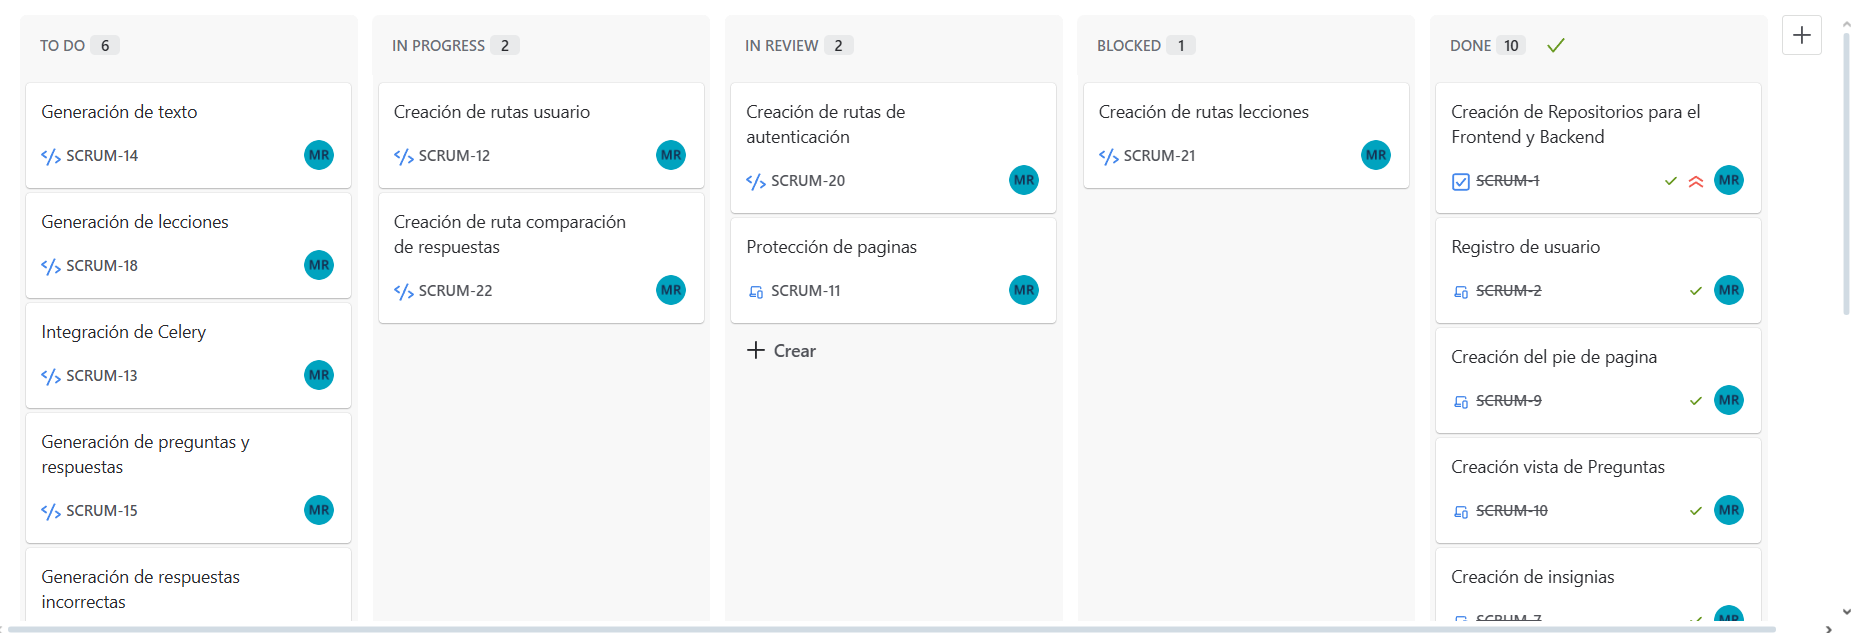
\includegraphics[width=1\linewidth]{Imagenes/tablero_tg.png}
  \caption{Tablero Scrumban}
  \label{fig:tablero}
\end{figure}

